\begin{center}
\rule{\textwidth}{0.5pt}
\end{center}
\begin{abstract}
The goal of this project is to develop a new approach to solve two well-known problems in robotics engineering: Path Planning and Trajectory Tracking for Automated Vehicles. Our novel approach introduced Artificial Potential Field and Genetic Algorithm to generate a collision-free Bezier spline-based trajectory for the automated vehicle. Then the PID control algorithm is used to help the car steer itself to follow the generated path from the starting point to the ending point.
\end{abstract}
\rule{\textwidth}{0.5pt}

\section{Introduction}
\subsection{Motivation and Purpose}
With the current technological trend, cars, robots, and vehicles have been able to move autonomously basically without any human interaction. Artificial intelligence is such a technology that has provided electric car auto-driving and complex problem solving capabilities to transport humans and objects to desired location. Having seen the vast potential in technological development, we chose Path Planning and Trajectory Tracking problems to start with with the hope of finding new solutions and being a motivational foundation for further researches from other engineers.

\begin{figure}[ht]
    \centering
    \begin{subfigure}[b]{0.45\textwidth}
        \centering
        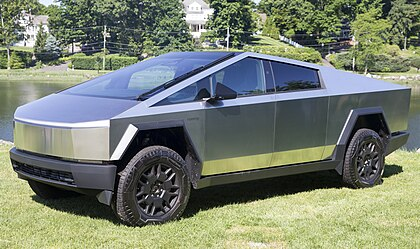
\includegraphics[width=\textwidth]{img/tesla_cybertruck.jpg}
        \caption{Tesla Cybertruck}
    \end{subfigure}
    \hfill
    \begin{subfigure}[b]{0.47\textwidth}
        \centering
        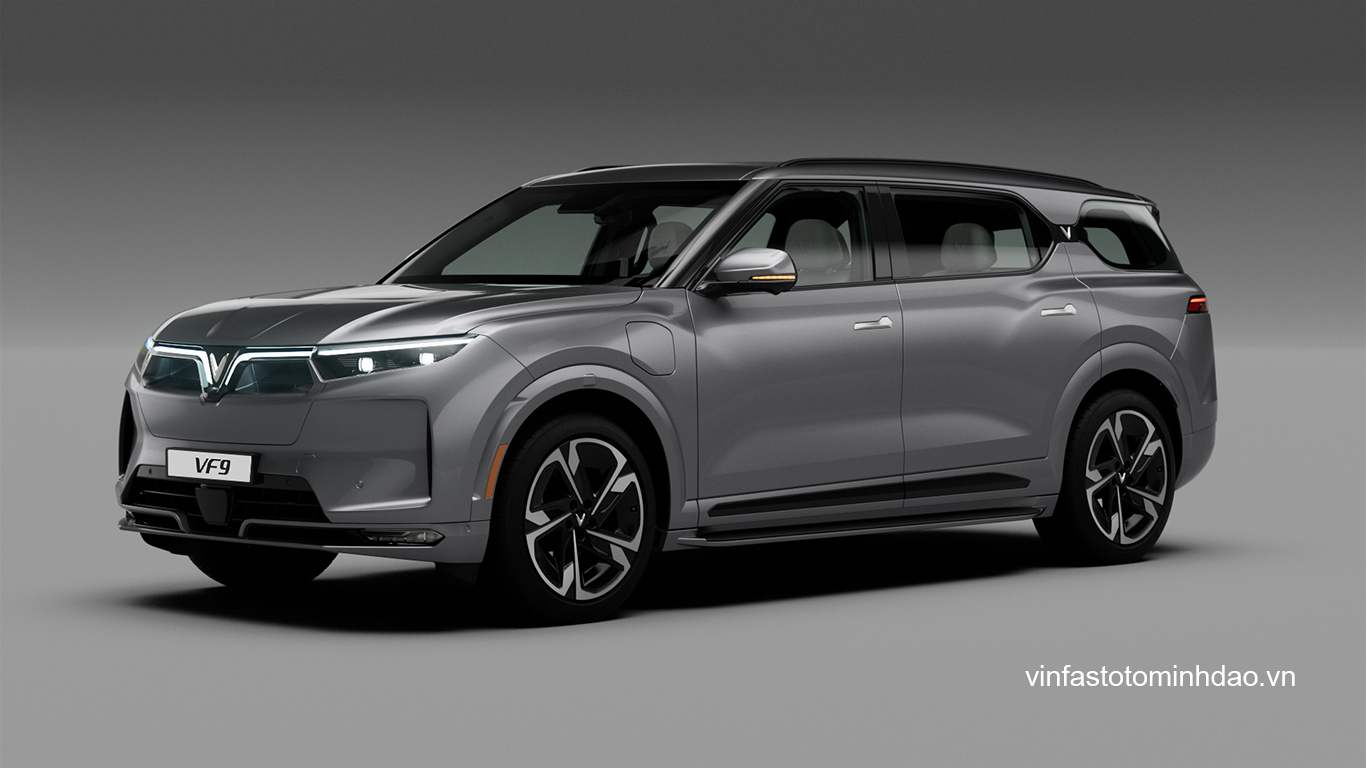
\includegraphics[width=\textwidth]{img/vinfast.jpg}
        \caption{Vinfast VF9}
    \end{subfigure}
    \caption{Electric Cars} % Overall caption
\end{figure}

\subsection{Goal}
    Currently, AI is the most robust tool to provide the self-driving capability for autonomous vehicles. However, since the technology requires data with high speciality such that it may become hard to obtain (data from specified sensors, high-cost peripherals and devices), we aim to achieve the collision-free motion using another way, which is Genetic Algorithm
